\begin{figure}[!htb]
\centering
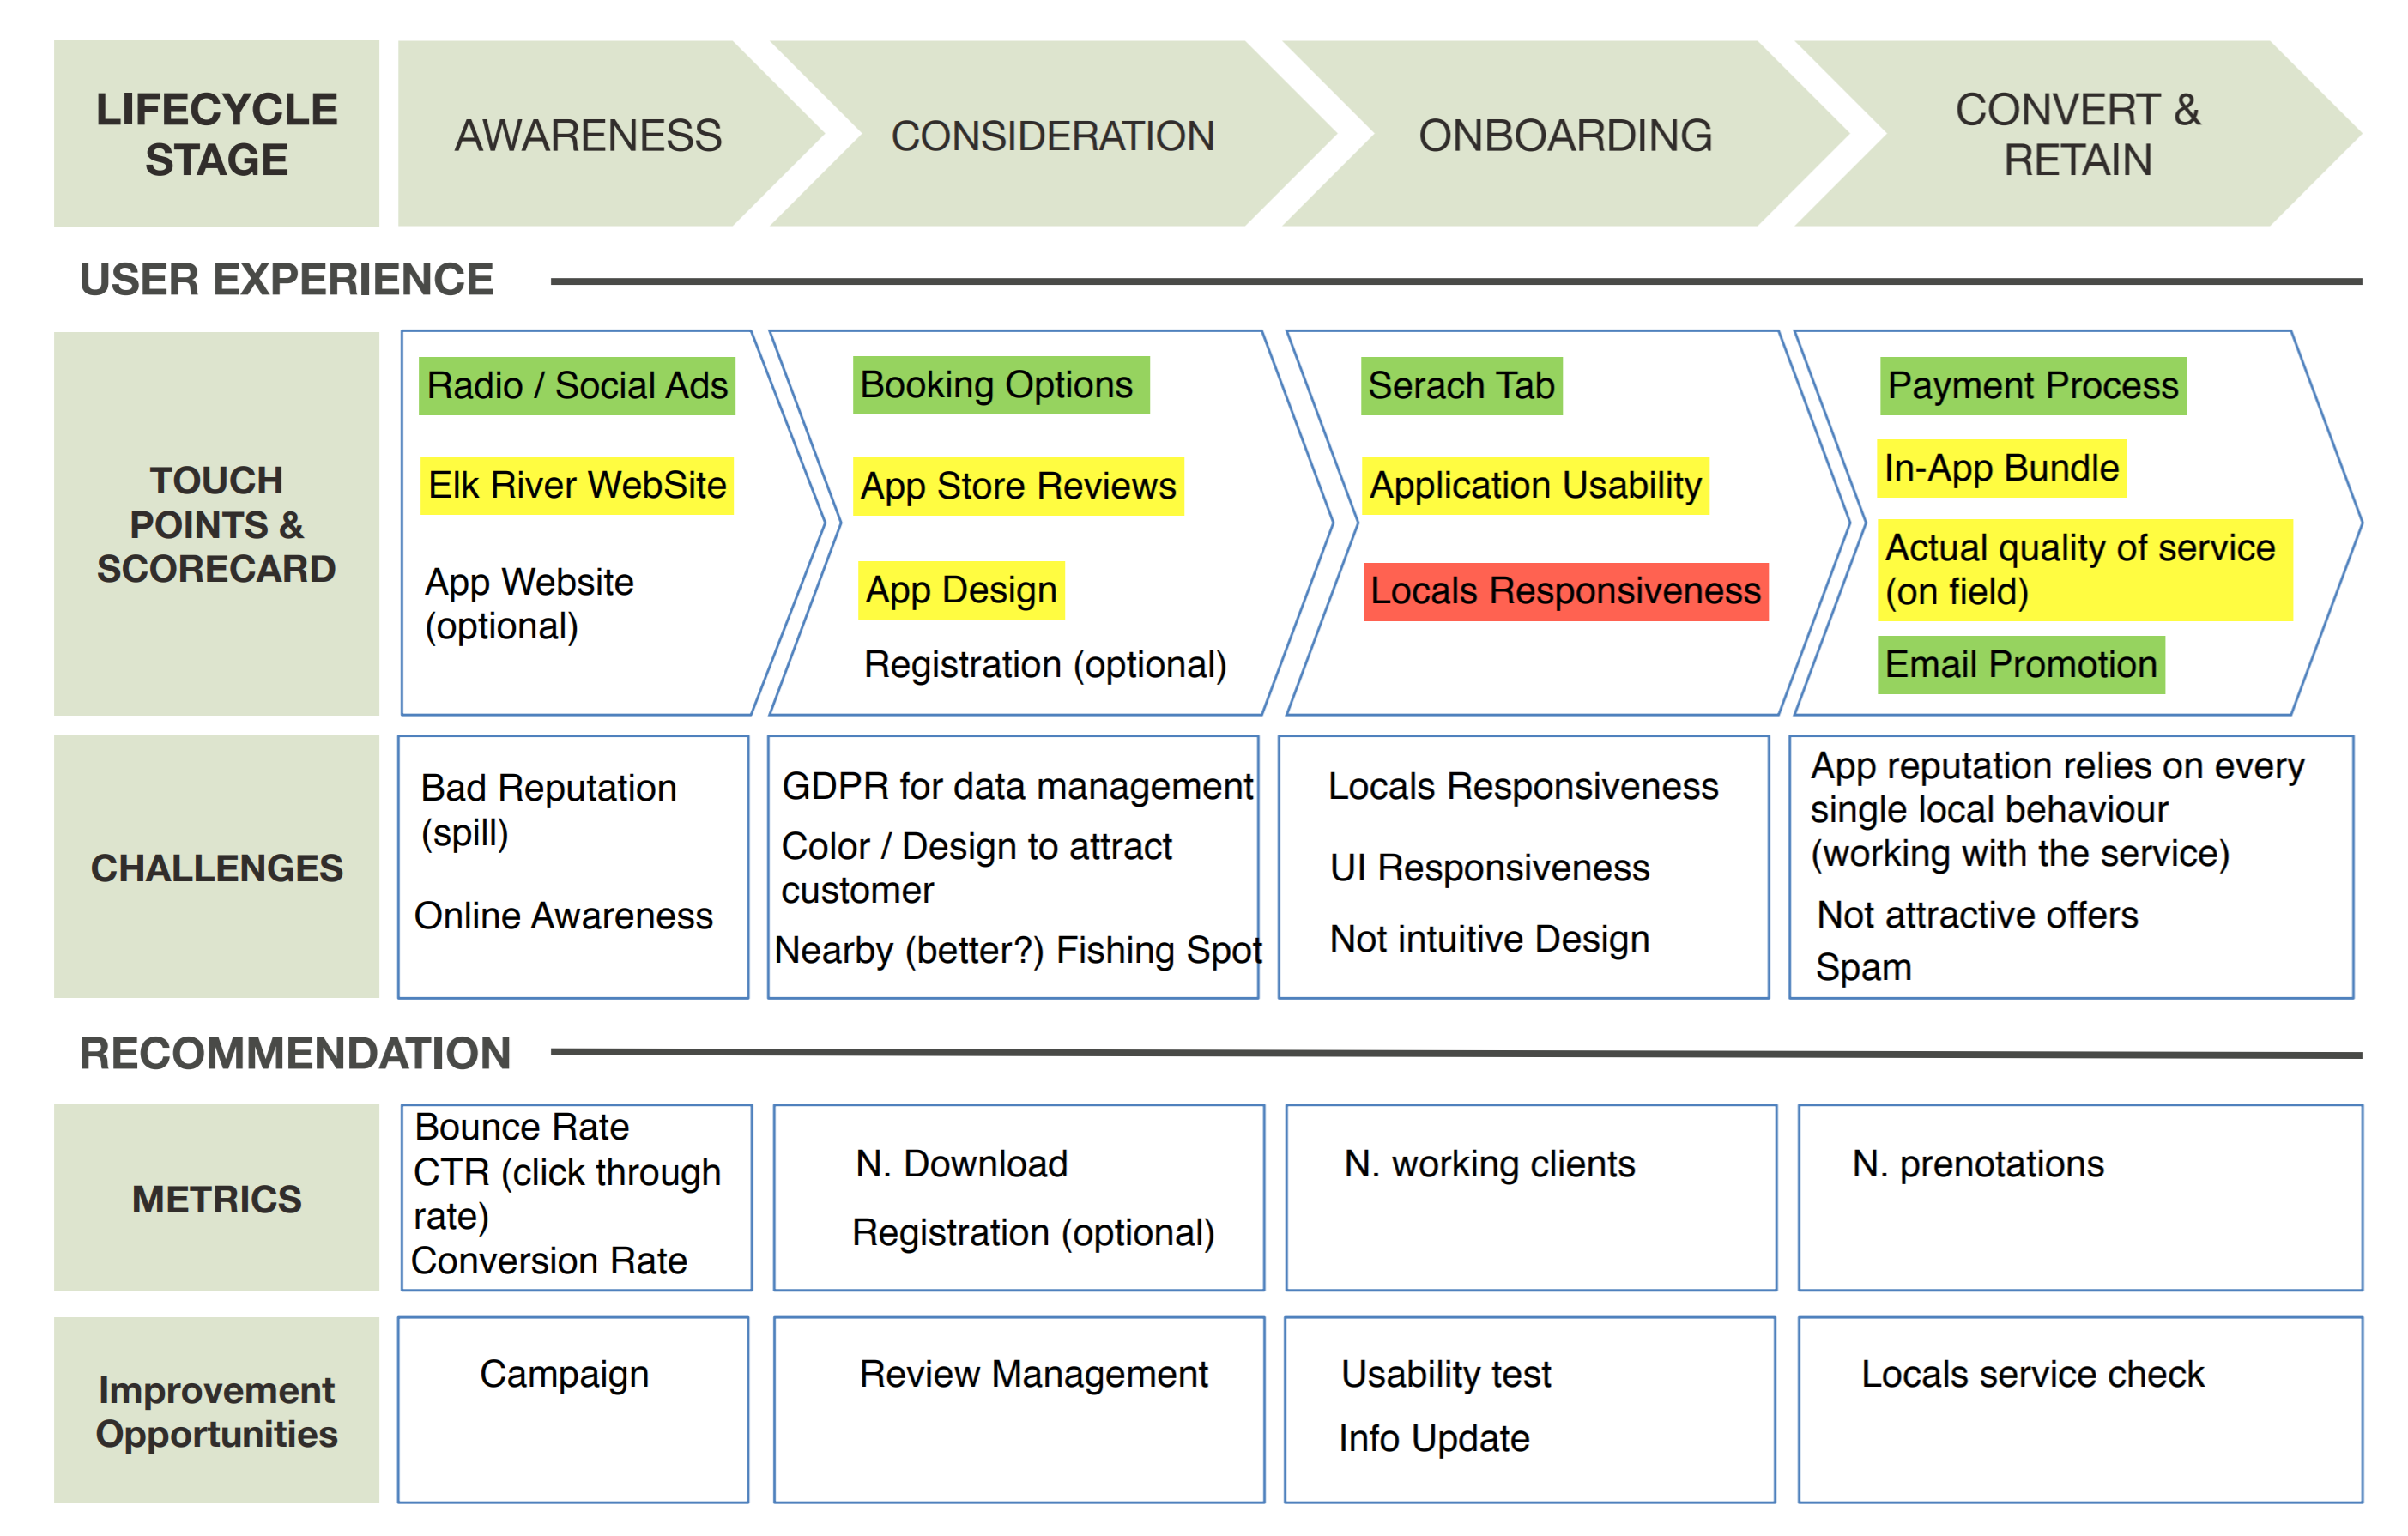
\includegraphics[width=1.0\textwidth]{Img/Customer_journey_map}
\caption{Customer journey map of a person who visits the area and uses services offered by locals}
\end{figure}

In the awareness phase, a potential customer becomes aware of the application existence. It is therefore important to find channels with biggest probability that a customer will notice the application. The easiest way to reach new customers is using social networks. Still, another channel very likely to succeed are radio stations in the area, since the majority of the persons traveling to the area will listen to some of these because, all of them being with excellent coverage. The Elk River website is a viable marketing channel as long as it is regularly updated with new information, inviting existing visitors to visit the website, and new visitors to search for information there. The spill of 2014 can be considered as the major challenge when bringing new visitors to the area but it is not something controllable. 

Most users with option to download an application first take into consideration the reviews of the application. They will read the application description, reviews and look at the application screenshots because they want to see what the application offers exactly. This application, being an application used for booking activities and places should present them in a clear way what are their options. Special attention must be payed to fulfill customers' needs from the beginning as this will make them spread the word. Bad reputation will for sure reject people from trying the application. Following good practices such as private data management is very important in today's ever growing concern for privacy.

After a user downloads the application and after verifying that the application look as expected, they will be able to see who are the locals offering services in the area. Therefore, it is important to bring as many locals as possible to use the application so that the visitors can immediately see the value in using the application. On our side, we need to make sure that the platform works as expected and that it is simple to use for everyone. 

After a user completes at least one booking using the application will they be able to give final verdict. Unfortunately, the quality of the service depend also on the real offer and so it is in the hands of the locals. Working with locals in the first period by giving them instruction how to improve could bring greater acquisition rate. Then, staying in touch with users by sending them promotional emails will make sure that they keep using the application.